\documentclass{iopart}
\usepackage{amssymb}
\usepackage{graphicx}
\usepackage{algorithmic}
\usepackage{algorithm}
\usepackage{url}
\usepackage{color}
%\usepackage{hyperref}
\newcommand{\mbf}[1]{\mathbf{#1}}
\newcommand{\mcl}[1]{\mathcal{#1}}
\newcommand{\msf}[1]{\mathsf{#1}}
\newcommand{\TODO}[1]{{\textcolor{red}{TODO: #1}}}
%\newcommand{\argmin}{\operatornamewithlimits{arg min}}
\newcommand{\argmin}{\mathrm{arg min}}
\newcommand{\ts}[1]{{\textstyle#1}}

\newcommand{\bq}{\begin{eqnarray}}
\newcommand{\eq}{\end{eqnarray}}
\newcommand{\diag}{\mathrm{diag}}

\newtheorem{theorem}{Theorem}[section]
\newtheorem{lemma}[theorem]{Lemma}
\newtheorem{proposition}[theorem]{Proposition}
\newtheorem{corollary}[theorem]{Corollary}

\newenvironment{proof}[1][Proof]{\begin{trivlist}
\item[\hskip \labelsep {\bfseries #1}]}{\end{trivlist}}
\newenvironment{definition}[1][Definition]{\begin{trivlist}
\item[\hskip \labelsep {\bfseries #1}]}{\end{trivlist}}
\newenvironment{example}[1][Example]{\begin{trivlist}
\item[\hskip \labelsep {\bfseries #1}]}{\end{trivlist}}
\newenvironment{remark}[1][Remark]{\begin{trivlist}
\item[\hskip \labelsep {\bfseries #1}]}{\end{trivlist}}

\newcommand{\qed}{\nobreak \ifvmode \relax \else
      \ifdim\lastskip<1.5em \hskip-\lastskip
      \hskip1.5em plus0em minus0.5em \fi \nobreak
      \vrule height0.75em width0.5em depth0.25em\fi}




\begin{document}

\title[A penalty method for PDE-constrained optimization]{A penalty method for PDE-constrained optimization}
\author{Tristan van Leeuwen$^1$ and Felix J. Herrmann$^2$}
\address{$^1$Centrum Wiskunde \& Informatica. Science Park, Amsterdam, the Netherlands\\
$^2$ Dept. of Earth, Ocean and Atmospheric Sciences.\\2207 Main Mall, Vancouver, BC Canada V6T 1Z4.}
\ead{tleeuwen@eos.ubc.ca}

\begin{abstract}
We present a method for solving PDE constrained optimization problems
based on a penalty formulation. This method aims to combine advantages
of both full-space and reduced methods by exploiting a large
search-space (consisting of both control and state variables) while
allowing for an efficient implementation that avoids storing and
updating the state-variables. This leads to a method that has roughly
the same per-iteration complexity as conventional reduced approaches
while defining an objective that is less non-linear in the control
variable by implicitly relaxing the constraint. We apply the method to a
seismic inverse problem where it leads to a particularly efficient
implementation when compared to a conventional reduced approach as it
avoids the use of adjoint state-variables. Numerical examples illustrate
the approach and suggest that the proposed formulation can indeed
mitigate some of the well-known problems with local minima in the
seismic inverse problem.
\end{abstract}

\maketitle

\section{Introduction}
In parameter estimation, the goal is to infer physical parameters (e.g., density, soundspeed or conductivity) 
from partial measurements of solutions of a PDE that describes the physical process as a 
function of the paramater of interest (e.g., a wave-equation, ). These problems arise in many applications such as
geophysics \cite{Haber2004,Epanomeritakis08}, medical imaging \cite{Abdoulaev2005} and non-destructive testing.

For linear PDEs, the resulting optimzation problem (after discretization) can be written as
\bq
\label{eq:constr}
\min_{\mbf{m},\mbf{u}} \ts{\frac{1}{2}}||P\mathbf{u} - \mathbf{d}||_2^2 \quad 
\mbox{s.t.} \quad A(\mathbf{m})\mathbf{u} = \mathbf{q},
\eq
where $\mathbf{m}$ is the (gridded) parameter of interest, $\mathbf{u}$ is the field and $\mathbf{d}$ are
the input data. The matrix $P$ restricts the predicted field to the measurement locations. 
The matrix $A(\mathbf{m})\mathbf{u} = \mathbf{q}$ represents the discretized PDE and $\mbf{q}$ is the 
source function. 

Oftentimes, measurements are made from multiple independent experiments, 
in which case $\mathbf{u}$ is a block vector containing the fields for different experiments. 
For some applications, such as seismic inversion, $\mbf{m}$ may represent up to $\mcl{O}(10^9)$ unknowns 
while $\mbf{u}$ may easily represent $\mcl{O}(10^{17})$.

\subsection{All-at-once approach}
A popular approach to solving
these constrained problems is based on the corresponding Lagrangian:
\bq
\mcl{L}(\mbf{m},\mbf{u},\mbf{v})=  \ts{\frac{1}{2}}||P\mathbf{u} - \mathbf{d}||_2^2 
+ \mbf{v}^*\left(A(\mathbf{m})\mathbf{u} - \mathbf{q}\right),
\eq
where $^*$ denotes the complex-conjugate transpose.
A necessary condition for a solution to the constrained problem (\ref{eq:constr}) is that 
it is a stationary point of the Lagrangian. 
Such a stationary point may be found using a Newton-like method by repeatedly solving
the KKT system \cite{Haber2000}
\bq
\left(
\begin{array}{ccc}
\nabla^2_{\mbf{m}}\mcl{L}&\nabla^2_{\mbf{m},\mbf{u}}\mcl{L}&\nabla^2_{\mbf{m},\mbf{v}}\mcl{L}\\
\nabla^2_{\mbf{u},\mbf{m}}\mcl{L}&\nabla^2_{\mbf{u}}\mcl{L}&\nabla^2_{\mbf{u},\mbf{v}}\mcl{L}\\
\nabla^2_{\mbf{v},\mbf{m}}\mcl{L}&\nabla^2_{\mbf{v},\mbf{u}}\mcl{L}&\nabla^2_{\mbf{v}}\mcl{L}\\
\end{array}
\right)
\left(
\begin{array}{c}
\delta \mbf{m}\\
\delta \mbf{u}\\
\delta \mbf{v}\\
\end{array}
\right)=
-\left(
\begin{array}{c}
\nabla_{\mbf{m}}\mcl{L}\\
\nabla_{\mbf{u}}\mcl{L}\\
\nabla_{\mbf{v}}\mcl{L}\\
\end{array}
\right),
\eq
and updating $\mbf{m}:=\mbf{m} + \delta\mbf{m}$, etc.

An advantages of such an `all-at-once' approach are that it eliminates the need to
solve the PDEs explicitly. However, this approach is often unfeasible
for large-scale applications we have in mind because it involves simultaneously updating
(and hence storing) all the variables (up to $\mcl{O}(10^{17})$). 

\subsection{Reduced approach}
For large-scale applications, one usually considers a \emph{reduced} problem
\bq
\min_{\mbf{m}}\phi(\mbf{m}) = \ts{\frac{1}{2}}||P\overline{\mbf{u}}(\mbf{m}) - \mbf{d}||_2^2,
\label{eq:redL}
\eq
where $\overline{\mbf{u}}(\mbf{m}) = A(\mathbf{m})^{-1}\mathbf{q}$.
The resulting optimization problem has a much smaller dimension and can be solved using black-box 
non-linear optimization methods. The gradient and the (Gauss-Newton) Hessian of 
$\phi$ are given by

\bq
\nabla\phi(\mbf{m}) &=& G(\mbf{m},\overline{\mbf{u}})^*\overline{\mbf{v}},\\
\nabla^2\phi(\mbf{m}) &=& G(\mbf{m},\overline{\mbf{u}})^*A(\mbf{m})^{-*}P^*PA(\mbf{m})^{-1}G(\mbf{m},\overline{\mbf{u}})\nonumber\\
&& + K(\mbf{m},\overline{\mbf{v}})^*A(\mbf{m})^{-*}G(\mbf{m},\overline{\mbf{u}}) + G(\mbf{m},\overline{\mbf{u}})^*A(\mbf{m})^{-*}K(\mbf{m},\overline{\mbf{v}})\nonumber\\
&& + R(\mbf{m},\overline{\mbf{u}},\overline{\mbf{v}}).
\eq
where $\overline{\mbf{v}} = A(\mbf{m})^{-*}P^*\left(\mbf{d} - P\overline{\mbf{u}}\right)$ and 
\bq
G(\mbf{m},\mbf{u}) &=& \frac{\partial A(\mbf{m})\mbf{u}}{\partial \mbf{m}},\\
K(\mbf{m},\mbf{v}) &=& \frac{\partial A(\mbf{m})^*\mbf{v}}{\partial \mbf{m}},\\
R(\mbf{m},\mbf{u},\mbf{v}) &=& \frac{\partial G(\mbf{m},\mbf{u})^*\mbf{v}}{\partial \mbf{m}}.
\eq

The disadvantage of this approach is that it
requires the solution of the PDEs at each update, making it computationally very expensive. 
It also strictly enforces the constraint at each iteration, which might lead to a very
nonlinear problem in $\mbf{m}$. Moreover, the corresponding Hessian is typically a
dense matrix that cannot be stored and computing its action involves additional
PDE solves. Practical approaches are usually based on Quasi-Newton approximations of
the reduced Hessian.

\subsection{Contributions and outline}
In this paper we present an alternative to the reduced approach which
has a roughly equivalent per-iteration complexity in terms of PDE solves
and storage but retains some of the characteristics of the all-at-once
approach in the sense that it exploits a larger search space by not
enforcing the constraints at each iteration.

The approach is based on a \emph{penalty} formulation of the constrained problem,
the solution of which coincides with that of the constrained problem (\ref{eq:constr}) for an. 
appropriate choice of the penalty parameter.
Such a reformulations of the constrained problem are well-known, 
but for the sake of completeness we give a brief overview in section \ref{penalty}. The main contribution
of this paper is a solution strategy, which is based on the elimination of the state variable $u$ via
a \emph{variational projection} approach as detailed in section \ref{varpro}. The benefit of this approach is
that it effectively eliminates these variables from the optizatiom problem and thus greatly reduces the dimensionality
of the optimization problem. Due to the special structure of the problems under consideration, this elimination 
can be done efficiently, leading to a tractable algorith for large-scale problems. 
Contrary to the conventional \emph{reduced} approach, the resulting algorihtm does \emph{not} enforce the constraint
$c(m,u)$ at each iteration and arguably leads to a less non-linear problem in $m$. It is outside the scope of the current
paper to give a rigorous prove of this statement, but a case-study on a simple toy problem presented in section
 \ref{toy} gives an intuitive justification.

A detailed description of the proposed algorihtm is given in section \ref{algorithm}.
Here, we also compare the penalty approach to both the all-at-once and the
reduced approaches in terms of algorithmic complexity.

Numerical
examples on seismic inversion using both the penalty and reduced
formulations are given in section \ref{examples}.

Possible extensions and open problems are discussed in section
\ref{discussion} and section \ref{conclusion} gives the conclusions.

\subsection{Related work}
The proposed method is related to the \emph{equation-error} approach,
which is typically used to identify the control variable in diffusion
problems given a \emph{complete} measurement of the state: $\mbf{d} = \mbf{u}$ by
solving $A(\mbf{m})\mbf{u} = \mbf{q}$ for $\mbf{m}$ \cite{Richter1981,Banerjee2013}. 
Given \emph{partial} measurements of the state $\mbf{d} = P\mbf{u}$, the proposed method can be seen as a
way of bootstrapping this by first attempting to reconstruct the complete
state from the partial measurements. 

\section{Penalty methods}
\label{penalty}
A constrained optimization problems of the form (\ref{eq:constr})
can be recast as an unconstrained problem by introducing a positive penalty function $\pi$ as follows
\bq
\label{eq:penalty}
\min_{\mbf{m},\mbf{u}} \Phi_{\lambda} = \ts{\frac{1}{2}}||P\mathbf{u} - \mathbf{d}||_2^2 + \lambda\pi(\mbf{A}(\mbf{m})\mbf{u} - \mbf{q}).
\eq
The idea is that any departure from the constraint is penalized so that the solution of this 
unconstrained problem will coincide with that of the constrained problem when $\lambda$ is large enough.

\subsection{Quadratic penalty function}
A quadratic penalty function $\pi(\cdot) = \ts{\frac{1}{2}}||\cdot||_2^2$ leads to a differentiable 
unconstrained optimization problem (\ref{eq:penalty}) whose minimizer $\{\overline{\mbf{m}}_{\lambda},\overline{\mbf{u}}_{\lambda}\}$ coincides with the solution
of the constrained optimization problem (\ref{eq:constr}) when $\lambda \uparrow \infty$ \cite[Thm. 17.1]{Nocedal}. 
Practical algorithms rely on repeatedly solving the unconstrained problem for increasing values of $\lambda$.
A common concern with this approach is that the Hessian may become increasingly ill-conditioned 
for large values of $\lambda$ when there are fewer constraints than variables. For PDE-constrained 
optimziation problems in inverse problems, there are typically enough constraints to prevent this and we will
discuss this in more detail in section \ref{algorithm}.

\subsection{Exact penalty methods}
For non-smooth penalty functions, such as $\pi(\cdot) = ||\cdot||_1$, the minimizer of $\phi_{\lambda}$
is a solution of the constrained problem for \emph{any} $\lambda \geq \bar{\lambda}$ for some $\bar{\lambda}$
\cite[Thm. 17.3]{Nocedal}. In practice, a continuation
strategy is used to find a suitable value for $\lambda$. An advantage of this approach is that $\lambda$ does
not become arbritarily large and this this avoids the ill-conditioning problems mentioned above. A disadvantage
is that the resulting unconstrained problem is no longer differentiable. 
With large-scale applications in mind, we do not consider exact penalty methods any further in this paper.

\section{Variational projection}
\label{varpro}
Using a quadratic penalty function, the constrained problem (\ref{eq:constr}) is reformulated as

\bq
\label{eq:penalty}
\min_{\mbf{m},\mbf{u}} \Phi_{\lambda}(\mbf{m},\mbf{u}) = \ts{\frac{1}{2}}||P\mathbf{u} - \mathbf{d}||_2^2 + \ts{\frac{1}{2}}\lambda||\mbf{A}(\mbf{m})\mbf{u} - \mbf{q}||_2^2.
\eq
The gradient and Hessian are given by
\bq
\nabla\phi_{\lambda} =\left(\begin{array}{c}
\nabla_{\mbf{m}}\phi_{\lambda}\\
\nabla_{\mbf{u}}\phi_{\lambda}\\
\end{array}
\right)
= 
\left(\begin{array}{c}
\lambda G(\mbf{m},\mbf{u})^*\left(A(\mbf{m})\mbf{u} - \mbf{q}\right)\\
P^*(P\mbf{u} - \mbf{d}) + \lambda A(\mbf{m})^*(A(\mbf{m})\mbf{u} - \mbf{q})\\
\end{array}
\right),
\eq
and
\bq
\nabla^2\Phi_{\lambda} &=&
\left(
\begin{array}{cc}
\nabla_{\mbf{m}}^2\Phi_{\lambda}&\nabla_{\mbf{m},\mbf{u}}^2\Phi_{\lambda}\\
\nabla_{\mbf{u},\mbf{m}}^2\Phi_{\lambda}&\nabla_{\mbf{u}}^2\Phi_{\lambda}\\
\end{array}
\right),
\eq
where
\bq
\nabla_{\mbf{m}}^2\Phi_{\lambda}(\mbf{m},\mbf{u}) &=& \lambda (G(\mbf{m},\mbf{u})^*G(\mbf{m},\mbf{u}) + R(\mbf{m},\mbf{u},A(\mbf{m})\mbf{u}-\mbf{q})),\\
\nabla_{\mbf{u}}^2\Phi_{\lambda}(\mbf{m},\mbf{u}) &=&P^*P + \lambda A(\mbf{m})^*A(\mbf{m}),\\
\nabla_{\mbf{m},\mbf{u}}^2\Phi_{\lambda}(\mbf{m},\mbf{u}) &=&\lambda (K(\mbf{m},A(\mbf{m})\mbf{u}) + A(\mbf{m})^*G(\mbf{m},\mbf{u})).\\
\eq
Of course, optimization in the full $(\mbf{m},\mbf{u})$-space is not feasible for large-scale problems, so we 
eliminate $\mbf{u}$ using a \emph{variational projection} approach \cite{Aravkin2012c} to define a reduced problem:
\bq
\label{eq:redpenalty}
\min_{\mbf{m}} \phi_{\lambda}(\mbf{m}) = \Phi_{\lambda}(\mbf{m},\overline{\mbf{u}}(\mbf{m})),
\eq
where $\overline{\mbf{u}}_{\lambda}(\mbf{m}) = \argmin_{\mbf{u}} \Phi_{\lambda}(\mbf{m},\mbf{u})$.
We interpret the $\argmin$ in a loose sence, in that $\overline{\mbf{u}}_{\lambda}$ only needs to be
a local minimizer.

It is readily verified that the gradient and Hessian of $\phi_{\lambda}$ are given by 

\bq
\label{eq:gradpen}
\nabla\phi_{\lambda}(\mbf{m}) &=& \nabla_{\mbf{m}}\Phi_{\lambda}(\mbf{m},\overline{\mbf{u}}_{\lambda}),\\
\label{eq:hesspen}
\nabla^2\phi_{\lambda}(\mbf{m}) &=& \nabla_{\mbf{m}}^2\Phi_{\lambda}(\mbf{m},\overline{\mbf{u}}_{\lambda}) \nonumber\\
&&-\nabla_{\mbf{m},\mbf{u}}^2\Phi_{\lambda}(\mbf{m},\overline{\mbf{u}}_{\lambda})\left(\nabla_{\mbf{u}}^2\Phi_{\lambda}(\mbf{m},\overline{\mbf{u}}_{\lambda})\right)^{-1}\nabla_{\mbf{u},\mbf{m}}^2\Phi_{\lambda}(\mbf{m},\overline{\mbf{u}}_{\lambda}).
\eq
Note that $\nabla^2\phi_{\lambda}(\mbf{m})$ is the Schur complement of $\nabla^2\Phi_{\lambda}$.

In section \ref{algorithm} we will use these expressions to devise an algorithm to solve 
the unconstrained problem (\ref{eq:redpenalty}), but first we will show that minimizing $\phi_{\lambda}$ 
is equivalent to minimizing $\Phi_{\lambda}$

\begin{theorem}
A local minimizer $\overline{\mbf{m}}_{\lambda}$ of $\phi_{\lambda}$ together with the corresponding $\overline{\mbf{u}}_{\lambda} = \argmin_{\mbf{u}} \Phi_{\lambda}(\overline{\mbf{m}},\mbf{u})$,
are also a minimizer of $\Phi_{\lambda}$ and vice versa.
\end{theorem}
\begin{proof}
Since $\overline{\mbf{u}}_{\lambda}$ is assumed to be a local minimizer of $\Phi_{\lambda}(\mbf{m},\cdot)$, it satisfies 
the following optimality conditions:
\[
\nabla_{\mbf{u}}\Phi_{\lambda}(\mbf{m},\overline{\mbf{u}}_{\lambda}) = 0,
\]
and
\[
\nabla^2_{\mbf{u}}\Phi_{\lambda}(\mbf{m},\overline{\mbf{u}}_{\lambda}) \succ 0.
\]
Likewise, since $\overline{\mbf{m}}_{\lambda}$ is a local minimizer of $\phi_{\lambda}$, it satisfies
\[
\nabla_{\mbf{m}}\phi_{\lambda}(\overline{\mbf{m}}_{\lambda}) = 0,
\]
and
\[
\nabla^2_{\mbf{m}}\phi_{\lambda}(\overline{\mbf{m}}_{\lambda}) \succ 0.
\]
We have to show that the pair $(\overline{\mbf{m}}_{\lambda},\overline{\mbf{u}}_{\lambda})$ satisfy the first and second order
optimilaty conditions of $\Phi_{\lambda}$. From the expression for the gradient of $\phi_{\lambda}$ (\ref{eq:gradpen}) it follows immediately
that $\nabla\phi_{\lambda} = 0 \iff \nabla\Phi_{\lambda} = 0$.
Since $\nabla^2\phi_{\lambda}$ is the Schur complement of $\nabla^2\Phi_{\lambda}$ it follows
that $\nabla^2\phi \succ 0, \nabla^2_{\mbf{u}}\Phi \succ 0 \iff \nabla^2\Phi_{\lambda} \succ 0$ (cf. \cite[prop. 14.1]{Saad}).\qed
\end{proof}

Finally, we show that minimizing $\phi_{\lambda}$ is equivalent to minimizing $\phi$ as $\lambda \uparrow \infty$
via the following Theorem.

\begin{theorem}
A (local) minimizer of $\phi_{\lambda}$ satisfies the first and second order optimality conditions of $\phi$ up
to $\mcl{O}(\lambda^{-1})$.
\end{theorem}
\begin{proof}
The optimzation problem for $\overline{\mbf{u}}_{\lambda}$ has a closed-form solution 
\bq
\overline{\mbf{u}}_{\lambda} = \left(P^*P + \lambda A^*A \right)^{-1}\left(P^*\mbf{d} + \lambda A^*\mbf{q}\right),
\eq
which can be re-written as
\[
\overline{\mbf{u}}_{\lambda} = A^{-1}\left(I + \lambda^{-1}A^{-*}P^*PA^{-1}\right)^{-1}\left(\lambda^{-1}A^{-*}P^*\mbf{d} + \mbf{q}\right).
\]
For $\lambda > \sigma_{\max}(PA^{-1})$, we expand the inverse as $(I + \lambda^{-1}B)^{-1} \approx I - \lambda^{-1}B + \lambda^{-2}B^2 + \ldots$
and find that
\bq
\overline{\mbf{u}}_{\lambda} &=& A(\mbf{m})^{-1}\mbf{q}\nonumber\\
&&+ \lambda^{-1}\left(A^{*}A\right)^{-1}P^*\left(\mbf{d} - PA^{-1}\mbf{q}\right)\nonumber\\
&&- \lambda^{-2}\left(A^{*}A\right)^{-1}P^*P\left(A^{*}A\right)^{-1}P^*\mbf{d} + \mcl{O}(\lambda^{-3}),\\
&=& \overline{\mbf{u}} + \mcl{O}(\lambda^{-1}).
\eq
If we substitute this in the expression for the gradient of $\phi_{\lambda}$ we get
\bq
\nabla\phi_{\lambda}(\mathbf{m}) &=& \lambda G(\mbf{m},\overline{\mbf{u}}_{\lambda})^*\left(A(\mbf{m})\mbf{u}_{\lambda} - \mbf{q}\right)\nonumber\\
&=& G(\mbf{m},\overline{\mbf{u}})^*\overline{\mbf{v}}  + \lambda^{-1}G(\mbf{m},A^{-1}\overline{\mbf{v}})^*\overline{\mbf{v}} + \mcl{O}(\lambda^{-2}) \nonumber\\
&=& \nabla\phi(\mbf{m}) + \mcl{O}(\lambda^{-1}).
\eq
For the Hessian we find
\bq
\nabla^2\phi_{\lambda}(\mbf{m}) &=& \nabla^2\phi(\mbf{m}) + \mcl{O}(\lambda^{-1}).
\eq
Next, we need to show that 

By assumption, $\overline{\mbf{m}}_{\lambda}$ is a local minimizer of $\phi_{\lambda}$ so that $\nabla\phi(\overline{\mbf{m}}_{\lambda}) = 0$ and
$\nabla^2\phi(\overline{\mbf{m}}_{\lambda}) \succ 0$. If follows that
\[
\nabla\phi(\overline{\mbf{m}}_{\lambda}) = \mcl{O}(\lambda^{-1}).
\]

\[
\nabla^2\phi(\overline{\mbf{m}}_{\lambda}) = \mcl{O}(\lambda^{-1})
\]

\qed
\end{proof}
\section{Analysis of a toy problem}
\label{toy}
Before describing algorithms to minimize $\phi_{\mathrm{pen}}$, we will illustrate the potential benefits
of the penalty approach over the conventional reduced approach with the help of a toy problem with
\[
A(\mbf{m}) = 
\left(\begin{array}{cc}
\frac{1}{2}&\frac{1}{4}\\
\frac{1}{4}&1\\
\end{array}\right),\quad
q = \left(\begin{array}{c}
1\frac{3}{4}\\
2\frac{1}{4}\\
\end{array}\right).
\]
The solution in this case is $\overline{m} = (1,1)$ and $\overline{u} =
(1,1)$. We use a Gauss-Newton method to solve both (\ref{eq:redL}) and (\ref{eq:redP}), starting from $m = (2,2)$. We use $\lambda = 0.1$ for the penalty approach.
Figure \ref{fig:opt} (a) shows the solution paths and (c) shows the convergence in terms of $||r||_2$ and $||c||_2$ for both the reduced
(black) and penalty approaches (red). The penalty approach gets very
close to the optimal solution in one iteration while the reduced
approach takes a detour because it is forced to satisfy the constraint
$c(m,u)=0$ at each iteration. Another perspective is offered by plotting the objective functions corresponding to the reduced and penalty approaches as a function of $m$.
Figure \ref{fig:opt} (c) shows the reduced objective (\ref{eq:redL}) and (d) shows the penalty objective (\ref{eq:redP}). The reduced objective in this case is quite non-linear while the penalty objective is quadratic.
These plots illustrate that the penalty formulation can indeed lead to an objective function that is much better behaved.

\section{Algorihtms}
\label{algorithm}
In this section we develop a pratical algorithm for the minimization of $\phi_{\lambda}$ based 
on the ideas discussed in section \ref{varpro}. We slightly elaborate the notation by explicitly revealing the multi-experiment structure of the problem;
The matrix $A$ is a block-diagonal matrix with blocks $A_i(\mbf{m})$ for $i=1\ldots M$, $\mbf{u} = [\mbf{u}_1; \ldots; \mbf{u}_{M}]$, etc.
Of course, $\mbf{m}$ does not depend on the experiment index.

The basic structure of


\subsection{Computing the gradient and Hessian}
Evaluation of $\phi_{\lambda}$ and its derivatives requires the minimization of $\Phi_{\lambda}$ w.r.t. $\mbf{u}$. 
Because of the block-structure of the problem and the linearity in $\mbf{u}$ this can be achieved by solving the 
following overdetermined system for each $i$

\bq
\label{eq:u_pen}
\left(
\begin{array}{c}
\sqrt{\lambda} A_i(\mbf{m})\\
P
\end{array}
\right)
\mbf{u}_{i} = 
\left(
\begin{array}{c}
\sqrt{\lambda} \mbf{q}_{i}\\
\mbf{d}_{i}
\end{array}
\right).
\eq

Since both $A_i$ and $P$ are sparse, we can efficiently solve this via direct (QR-) factorization or using an iterative method like LSQR or LSMR \cite{Paige1982,Fong2011}.
Given these solutions $\{\mbf{u}_i\}$, the gradient and Gauss-Newton Hessian of $\phi_{\lambda}$ are given by (cf eq. \ref{eq:gradpen}-\ref{eq:hesspen})

\bq
\nabla{\phi}_{\lambda} &=& \sum_{i}\lambda G_{i}^*\left(A_i\overline{\mathbf{u}}_{i} - \mathbf{q}_{i}\right),\\
\nabla^2{\phi}_{\lambda} &=& \sum_{i}\lambda G_{i}^*G_{i} - \lambda^2G_{i}^*A_i\left(P^*P + \lambda A_i^*A_i \right)^{-1}A_i^*G_{i}\nonumber\\
&=&\lambda\sum_{i}G_{i}^*G_{i} - G_{i}^*\left(I + \lambda^{-1}A_i^{-*}P^*PA_i^{-1} \right)^{-1}G_{i},
\eq
where $G_{i} = \frac{\partial A_i(\mbf{m})\overline{\mbf{u}}_{i}}{\partial \mbf{m}}$, which is typically a sparse diagonally dominant matrix.

\subsection{Contination of $\lambda$}

\subsection{Complexity estimates}
Assuming we can solve equations (\ref{eq:u_pen}) and (\ref{eq:u_red})
equally efficient, the penalty-based method requires a factor of 2 less
computation and storage. Note, however, that for the penalty-based
formulation we get an (approximate) Newton method while the reduced
method only uses a Quasi-Newton approach. A Gauss-Newton method for the
reduced approach would require far more PDE-solves and is not considered
here. A summary of the leading order computational costs of the penalty, reduced and all-at-once approaches is given in table \ref{table:costs}.

\section{Numerical experiments}
\label{examples}
For the examples, we discretize the 2D Helmholtz operator using a
5-point finite-difference stencil with absorbing boundary conditions.
The Quasi-Netwon algorithm \ref{QN2} is augmented with a simple
back-tracking linesearch to ensure descent.


\section{Discussion}
\label{discussion}
This paper lays out the basics of an efficient implementation of the
penalty method for PDE-constrained optimization. A few remaining issues
and possible extensions are listed below.
\begin{description}

\item[Solving large, sparse, mildly overdetermined systems] 
A key step in the penalty method is the solution of the augmented PDE
(\ref{eq:u_pen}). While we can make use of factorization techniques for
small-scale applications, industry-scale applications will typically
require (preconditioned) iterative solution of such systems. A promising
candidate is a generic accelerated row-projected method described by
\cite{Bjorck1979,Gordon2013} which proved successful in seismic
applications and can be easily extended to deal with overdetermined
systems \cite{Censor1983}.

\item[Time-domain formulation]
We have described application of the penalty method to a formulation in
the frequency domain, in which case we can hope to store a complete
wavefield $\mathbf{u}_{kl}$ for one source and frequency. In a
time-domain formulation, the PDE (after spatial discretization) can be
written as
 \[
 M(\mathbf{m})\mbf{u}'(t) + S\mathbf{u}(t) = \mathbf{q}(t),
 \]
which can be solved via some form of time-stepping. The augmented
wave-equation involves an extra equation of the form $P\mathbf{u}(t) =
\mbf{d}(t)$. While we can in principle form a large overdetermined system
for the wavefield at all timesteps, this is not feasible and a suitable
time-stepping strategy will have to be developed to solve the augmented
PDE without storing the wavefields for all timesteps.

\item[Other PDE-constrained optimization problems]
The penalty formulation can be applied to any PDE-constrained
optimization problem. We can only expect an efficient implementation
along the lines described in this paper, however, if the PDE is linear
in the state variable. In particular, application to multi-parameter
seismic inversion (e.g., visco-acoustic, variable density,
visco-elastic) is straightfoward.

\item[Dimensionality reduction]
The computational cost may be reduced by using recently proposed
dimensionality reduction techniques that essentially reduce the number
of right-hand-sides of the PDE by random subselection or aggregration
\cite{Haber2012,Friedlander2012,VanLeeuwen2012b}. These techniques can
be directly included in the penalty formulation by introducing new
sources and their corresponding data;
\[
\widetilde{\mbf{q}}_{kl'} = \sum_{l}w_{ll'}\mbf{q}_{kl}, \quad \widetilde{\mbf{d}}_{kl'} = \sum_{l}w_{ll'}\mbf{d}_{kl},
\]
where $l' = [1,2,\ldots,N_s']$ ($N_s' << N_s$) and $w_{l'l}$ are
suitably chosen random weights.

\item[Regularization] 
Regularization penalties on the model $\mathbf{m}$ can be included in
a trivial manner. Also, regularization techniques on the (Gauss-Newton)
subproblems can be included. This includes for example $\ell_1$
regularization as proposed by \cite{Li2012} and $\ell_2$ regularization
as is used in trust-region methods. 

\item[Penalties] 
Penalties other than the $\ell_2$ norm on either the data-misfit or the
constraint can be included in the formulation (\ref{eq:penalty}).
However, this will most likely prevent us from solving for the
wavefields efficiently via system of equations (\ref{eq:u_pen}). Still,
most alternative penalties may be approximated by a weighted $\ell_2$
norm, in which case a system like (\ref{eq:u_pen}) \emph{can} be formed 
and solved via an iteratively re-weighted least-squares approach \cite{Bjorck1979}.

\item[Nuisance parameters] 
Formulations of the inverse problem may include additional
parameters that need to be estimated. An example of this are the
source-weights in the seismic applications. The penalty objective, in
this case becomes
\[
\phi_{\lambda}(\mathbf{m},\mathbf{u},\theta) = \ts{\frac{1}{2}}\sum_{k,l}||\theta_{kl}P \mbf{u}_{kl} - \mbf{d}_{kl}||_2^2 + \lambda^2||\theta_{kl}A_k(\mbf{m})\mbf{u}_{kl} - \mbf{q}_{kl}||_2^2,
\]
The wavefield may be solved first from (\ref{eq:u_pen}) and subsequent
minimization over $\theta$ for the given wavefields is trivial as a
closed-form solution is available:
\[
\theta_{kl} = \frac{\mbf{u}_{kl}^*\left(P^*\mbf{d}_{kl} + \lambda^2A_k^*\mbf{q}_{kl}\right)}{||P\mbf{u}_{kl}||_2^2 + \lambda^2 ||A_k\mbf{u}_{kl}||_2^2}.
\]

This approach can be generalized to more complicated situations in which
a closed-form solution is not available \cite{Aravkin2012c}.

\item[Contination strategies for $\lambda$] 
The experiments presented in this paper were done for a fixed value of
$\lambda$. To ensure that one really solves the original constrained
problem, however, a suitable strategy for increasing $\lambda$ needs to
be developed.

\item[Optimization strategies]
In this paper we described a Gauss-Newton method to minimize the reduced
penalty objective (\ref{eq:redpenalty}). Using the expressions for the gradient and Hessian presented in section 3.1, we can design other Newton variants. 

Recently proposed stochastic algorithms aimed at dramatically reducing the cost of PDE-constrained optimization problems by working on a small subsets of the right-hand-sides \cite{Krebs09,Friedlander2012,Haber12,VanLeeuwen2012b} are directly applicable to this formulation.

\end{description}

\section{Conclusions}
\label{conclusion}
We have presented a new method for PDE-constrained optimization based on
a penalty formulation of the constrained problem. The method
relies on solving for the state variables from an augmented system that
is comprised of the original discretized PDE and the measurements. The
resulting estimates of the state variables can be used to directly
estimate the control variable from the PDE via an equation-error
approach. The main benefits of this method are: \emph{i)} The state
variables for each experiment can be obtained independently and do not
have to be stored or updated as part of an iterative optimization
procedure, \emph{ii)} the penalty formulation leads to a less non-linear
formulation than the reduced approach where the PDE-constraint is
eliminated explicitly, and \emph{iii)} the gradient of the objective
with respect to the control variable can be computed directly from the
state variables, without the need to solve adjoint PDEs. We illustrate
the approach on a non-linear seismic inverse problem, showing that the
reduced non-linearity leads to significantly better results than the
reduced approach at roughly half the computational costs (due to the
fact that there is no adjoint equation to solve). Moreover, the penalty
approach succesfully mitigates some of the the issues with local minima
making the procedure less sensitive to the initial model.

\section*{Acknowledgments}
The authors wish to thank Dan and Rachel Gordon for valuable discussions
on the CARP-CG method. This work was in part financially supported by
the Natural Sciences and Engineering Research Council of Canada
Discovery Grant (22R81254) and the Collaborative Research and
Development Grant DNOISE II (375142-08). This research was carried out
as part of the SINBAD II project with support from the following
organizations: BG Group, BGP, BP, Chevron, CGG, ConocoPhillips, ION,
Petrobras, PGS, Total SA, WesternGeco and Woodside.


\clearpage

\begin{table}
\begin{tabular}{c|c|c|p{5cm}}
         & \# PDE's & Storage & Gauss-Newton update \\
\hline
penalty  &  $N_s \times N_f $  &    $N_g$     & solve sparse SPSD system  in $N_g$ unknowns \\
\hline
reduced  &  $2(N_s \times N_f) $  &    $2N_g$     & solve matrix-free linear system in $N_g$ unknowns, requires $N_f \times N_s$ per mat-vec                   \\
\hline
all-at-once&   0   &    $N_f \times N_s \times N_g$   &  solve sparse symmetric, possibly indefinite system in $(N_f + N_s + 1) \times N_g$ unknowns \\ 
\end{tabular}
\caption{Leading order computation and storage costs per iteration of different methods; $N_s$ denotes the number of sources, $N_f$ denotes the number of frequencies and $N_g$ denotes the number of gridpoints.
for large-scale seismic inverse problems we typically have $N_s = \mcl{O}(10^6)$, $N_f = \mcl{O}(10^1)$ and $N_g = \mcl{O}(10^9)$}
\label{table:costs}
\end{table}
\clearpage

\begin{algorithm}
\caption{Gauss-Newton algorithm based on the penalty formulation}
\label{GN1}
\begin{algorithmic}
\FOR{$t = 0$ to $N$}
\STATE $\mbf{g}_t = 0$
\STATE $H_t = 0$
\FOR{$k = 1$ to $N_f$}

\FOR{$l = 1$ to $N_s$}
\STATE solve $\left(\begin{array}{c} \lambda_t A_k(\mbf{m}_t) \\ P \end{array}\right)\mbf{u}_{kl} = \left(\begin{array}{c}\lambda_t\mbf{q}_{kl}\\ \mbf{d}_{kl} \end{array}\right)$
\STATE $\mbf{g}_t = \mbf{g}_t  + \lambda_t^2G_k(\mbf{m}_t, \mbf{u}_{kl})^*(A_k(\mbf{m}_t)\mbf{u}_{kl} - \mbf{q}_{kl})$
\STATE $H_t = H_t + (\lambda_t^2 - 1)G_k(\mbf{m}_t, \mbf{u}_{kl})^*G_k(\mbf{m}_t, \mbf{u}_{kl})$
\ENDFOR


\ENDFOR

\STATE solve $H_t\Delta \mbf{m}_t = -\mbf{g}_t$
\STATE update $\mbf{m}_{t+1} = \mbf{m}_t + \Delta \mbf{m}_t$
\STATE update $\lambda_t$.
\ENDFOR
\end{algorithmic}
\end{algorithm}

\begin{algorithm}
\caption{Quasi-Newton algorithm based on the reduced formulation}
\label{QN2}
\begin{algorithmic}
\FOR{$t = 0$ to $N$}
\STATE $\mbf{g}_t = 0$
\FOR{$k = 1$ to $N_f$}

\FOR{$l = 1$ to $N_s$}
\STATE solve $A_k(\mbf{m}_t)\mbf{u}_{kl} =\mbf{q}_{kl}$
\STATE solve $A_k(\mbf{m}_t)^*\mbf{v}_{kl} = -P^*(P\mbf{u}_{kl} - \mbf{d}_{kl})$
\STATE $\mbf{g}_t = \mbf{g}_t  + G_k(\mbf{m}_t, \mbf{u}_{kl})^*\mbf{v}_{kl}$
\ENDFOR

\ENDFOR

\STATE apply L-BFGS Hessian $\Delta \mbf{m}_t = \msf{lbfgs}(-\mbf{g}_t,\{\mbf{m}_{t-M}, \ldots, \mbf{m}_t\},\{\mbf{g}_{t-M}, \ldots, \mbf{g}_t\})$
\STATE find a suitable steplength $\alpha$ 
\STATE update $\mbf{m}_{t+1} = \mbf{m}_t + \alpha\Delta \mbf{m}_t$
\ENDFOR
\end{algorithmic}
\end{algorithm}


\clearpage

\begin{figure}
\centering
\begin{tabular}{cc}
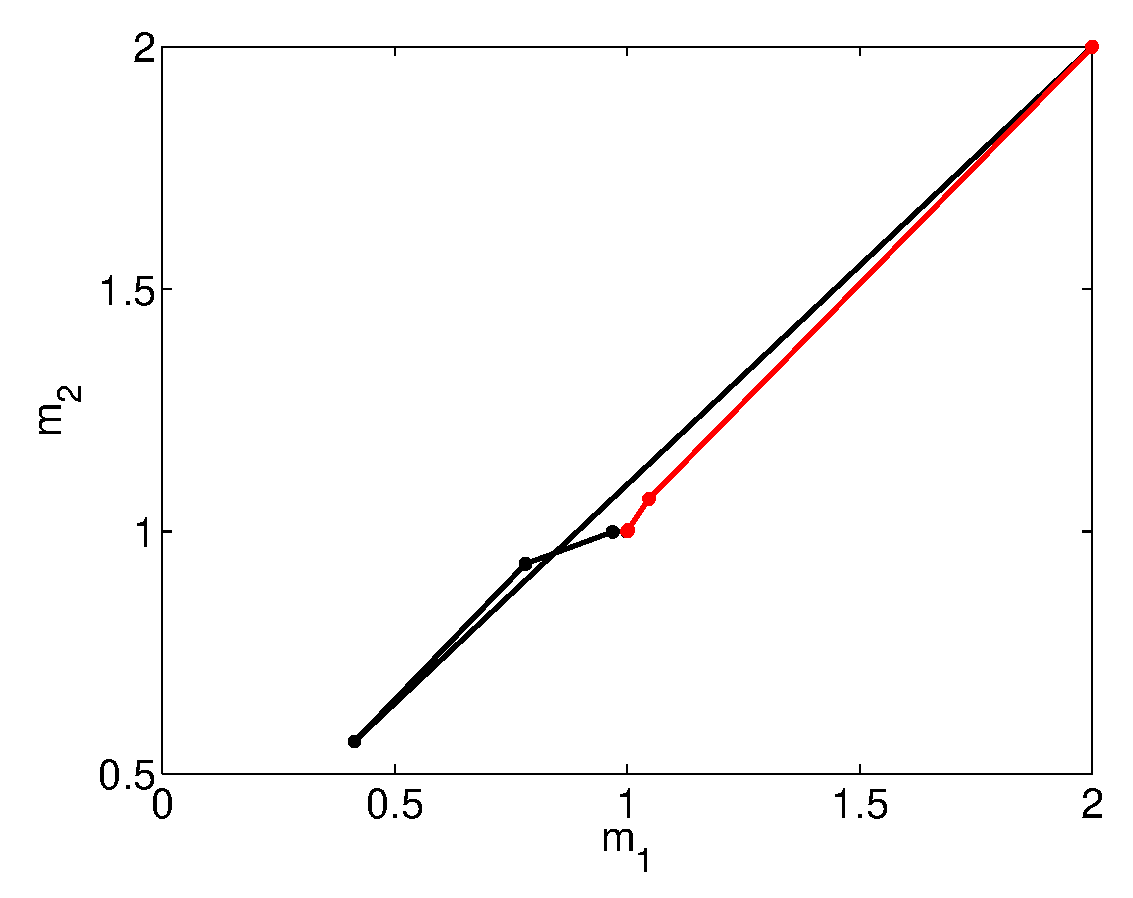
\includegraphics[scale=.4]{./figs/opt_b}&
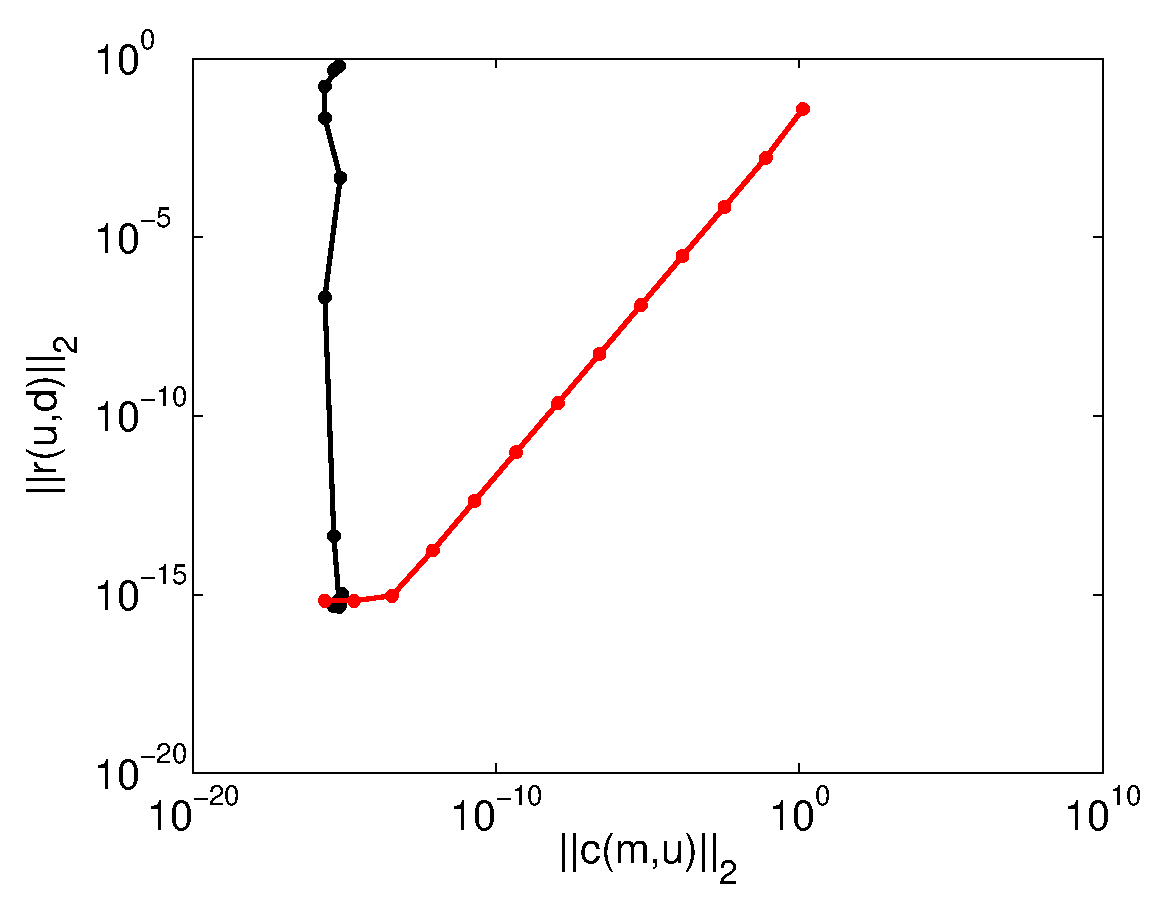
\includegraphics[scale=.4]{./figs/opt_c}\\
{\small (a)}&{\small (b)}\\
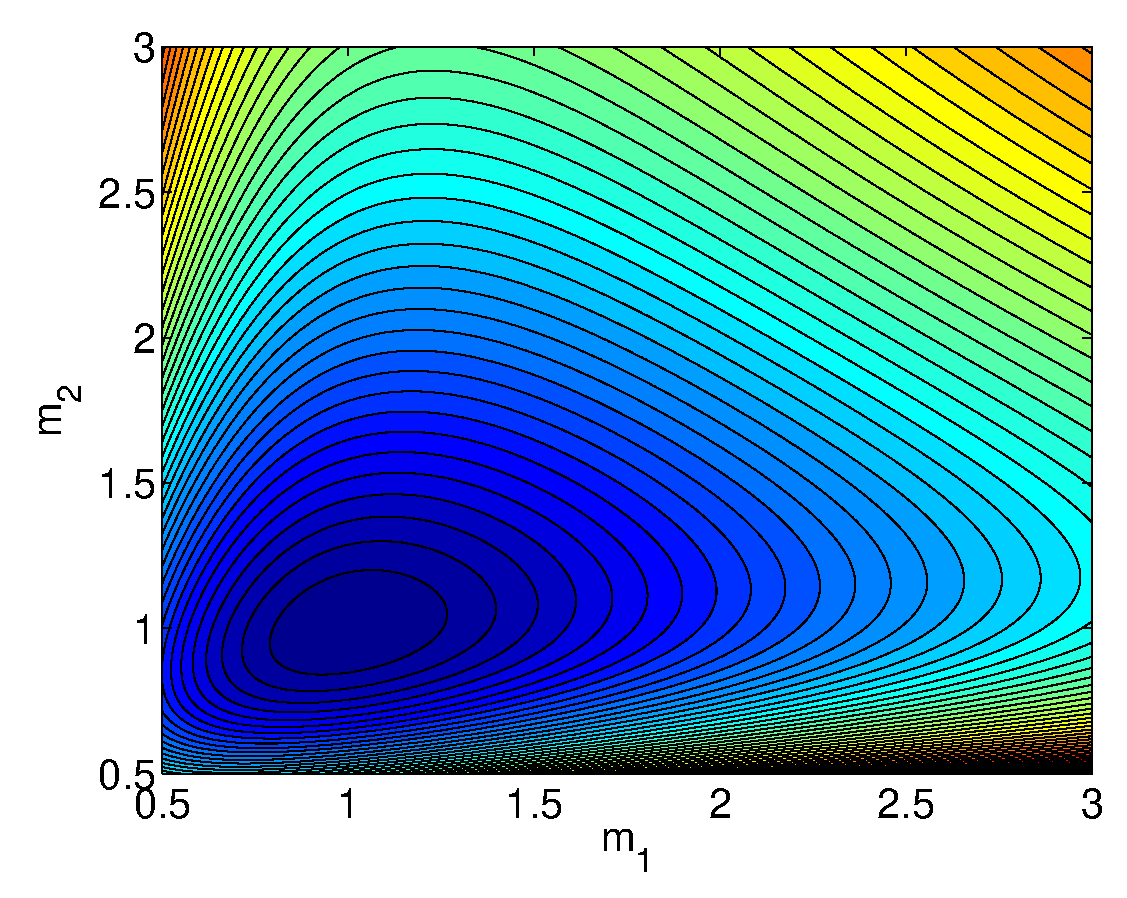
\includegraphics[scale=.4]{./figs/opt_d}&
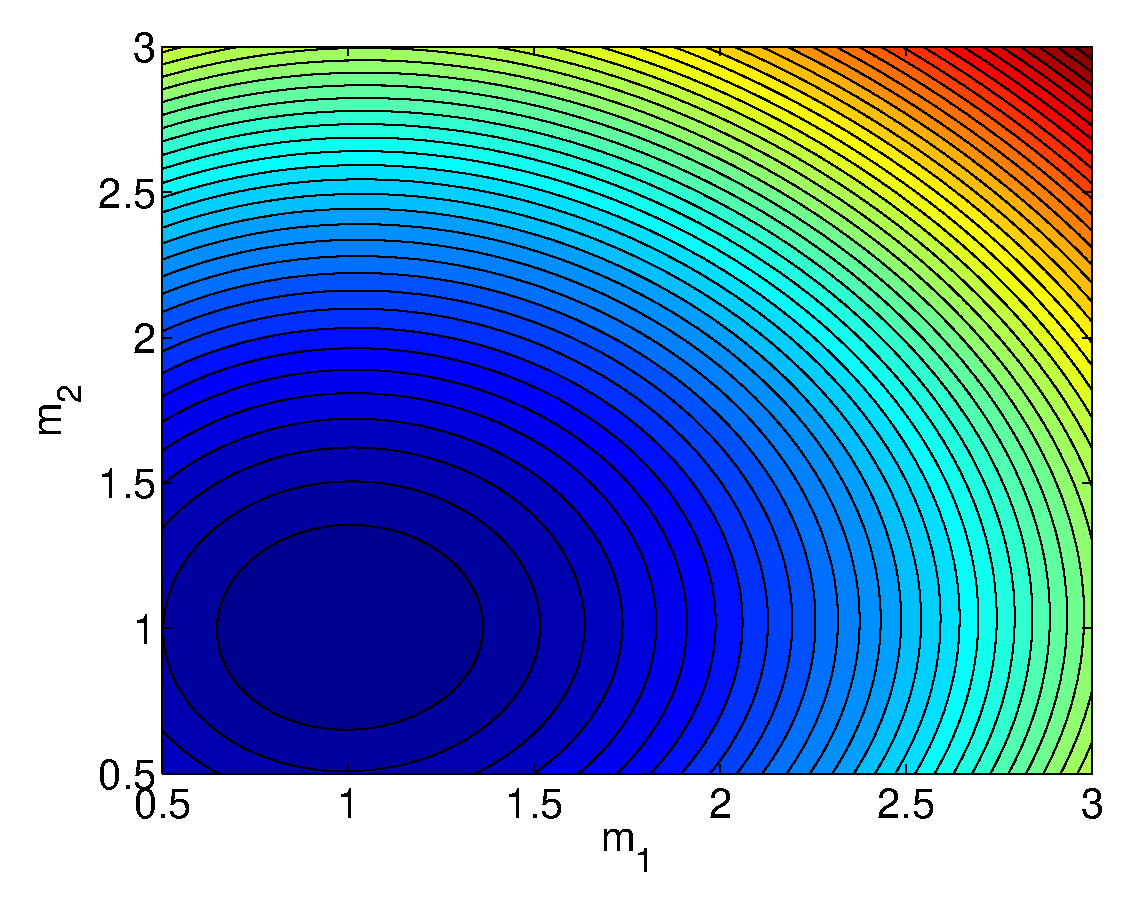
\includegraphics[scale=.4]{./figs/opt_e}\\
{\small (c)}&{\small (d)}\\
\end{tabular}
\caption{Illustration of the reduced and penalty approach on a simple 4 dimensional test problem. (a) Solution paths and (b) the convergence in terms of $||r||_2$ and $||c||_2$ for both the reduced (black) and penalty approaches (red). The objective functions corresponding to the reduced and penalty approaches are shown in (c) and (d) respectively.}
\label{fig:opt}
\end{figure}



\clearpage
\bibliographystyle{unsrt}
\bibliography{mybib}



\end{document}